%%%%%%%%%%%%%%%%%%%%%%%%%%%%%%%%%%%%%%%%%%%%%%%%%%%%%%%%%%%%%%%%%%%%%%%%
\chapter{Magnetic Resonance Imaging} \label{chap:MagneticResonanceImaging}
%%%%%%%%%%%%%%%%%%%%%%%%%%%%%%%%%%%%%%%%%%%%%%%%%%%%%%%%%%%%%%%%%%%%%%%%
\vspace{1cm}

Magnetic resonance imaging (MRI) is one of the most powerful and versatile techniques in modern medical imaging. Its non-invasive nature and the absence of ionizing radiation have established it as a cornerstone in both clinical diagnostics and biomedical research. MRI exploits the fundamental physical interactions between nuclear spins and magnetic fields, providing not only high-resolution structural images, but also access to functional, metabolic, and microstructural information.

This chapter goes through the fundamental concepts of MRI. First, it introduces the underlying physical principles of nuclear magnetic resonance, including spin dynamics, relaxation processes, and signal generation. Second, it describes how spatial encoding is achieved through magnetic field gradients, which allow the reconstruction of three-dimensional images.

\section{Physical Principles}
Magnetic resonance imaging (MRI) is based on the fundamental physical phenomenon of nuclear magnetic resonance (NMR), first demonstrated experimentally by I.\ Rabi in 1938 and later independently verified by Purcell and Bloch in 1946\,\cite{NMR}. NMR describes the resonant interaction between the intrinsic magnetic moment of atomic nuclei and external magnetic fields. This effect enables the observation of nuclear spin behavior through the emission of electromagnetic radiation, providing the physical foundation for MRI, a technique capable of generating high-resolution, non-invasive images of biological tissues.

If a nucleus possesses an intrinsic angular momentum, or spin \vect{I}, the associated magnetic dipole moment is:
\begin{equation}
    \bm{\upmu} = \gamma \vect{I},
\end{equation}
where $\gamma$ is the gyromagnetic ratio, a constant depending on the nucleus species. Only nuclei with a nonzero spin quantum number can exhibit magnetic resonance. Actually, nuclei with a integer spins are not able to produce detectable signals in MRI, because their gyromagnetic ratios are much smaller than those of half-integer spins. Among them, in biological tissues, the hydrogen nucleus ($^1$H) is the most suitable for MRI because of its high abundance in water and lipids and its relatively large $\gamma$, which yields strong detectable signals.

The result of an observation of the $z$-component of the angular momentum \vect{I} of a single nucleus in its ground state is an integer or half-integer number $m$ ranging from $-I$ to $+I$, in steps of \num{1}. Thus, $m$ can assume $2I + 1$ distinct values, which implies $2I + 1$ possible values for the measurement of the $z$-component of the magnetic moment
\begin{equation}
    \mu_z = \gamma \hbar m,
\end{equation}
where $\hbar$ is the reduced Planck constant.

Each value of $m$ corresponds to a specific energy level of the nucleus. When a magnetic field $\vect{B_0}$ is applied, these energy levels split due to the Zeeman effect, resulting in a set of discrete energy states. The energy associated with each state is given by
\begin{equation}
    E_m = -\gamma \hbar m B_0.
\end{equation}
In case of $^1$H, which has $I = \frac{1}{2}$, the two possible values of the magnetic moment correspond to $m = +\frac{1}{2}$ and $m = -\frac{1}{2}$. This results, in turn, in two distinct energy states separated by $\Delta E = \gamma \hbar B_0$. The presence of discrete energy levels generates an observable quantity named magnetization \vect{M}, which is defined as
\begin{equation}
    \vect{M} = N \gamma \hbar (\langle I_x \rangle \vect{i} + \langle I_y \rangle \vect{j} + \langle I_z \rangle \vect{k}),
\end{equation}
where $N$ is the number of nuclei with nonzero spin, and $\langle \cdot \rangle$ denotes the expectation values of the nuclear spin components along the axes. At relatively low temperature $T$ (even room temperature) and high magnetic field \vect{B_0}, the magnetization obeys Curie's law\,\cite{curie_law}:
\begin{equation}
    \vect{M} = N\frac{\gamma^2 \hbar^2 I(I+1)}{3\mathrm{k}_\mathrm{B} T} \vect{B_0},
\end{equation}
where $\mathrm{k}_\mathrm{B}$ is the Boltzmann constant. It is important to notice that stronger magnetic fields or lower temperatures increase the detectable magnetization.

The last fundamental principle of NMR is a phenomenon, known as Larmor precession, which originates from the application of an external magnetic field to nuclei with nonzero spin. The magnetic moments $\bm{\upmu}$ of the nuclei will not just align with the magnetic field, but they will describe a conical motion around \vect{B_0} (Fig.\,\ref{fig:larmor_precession}), at the Larmor frequency:
\begin{equation}
    \nu_\textrm{L} = \frac{\omega_\textrm{L}}{2\uppi} = \frac{\gamma B_0}{2\uppi}.
\end{equation}
To perturb the equilibrium state and generate a measurable signal, a second oscillating magnetic field \vect{B_1}, also called radiofrequency (RF) pulse, is applied perpendicularly to \vect{B_0}. If the oscillation frequency of \vect{B_1} matches $\omega_\mathrm{L}$, resonance occurs and the nuclei absorb energy, undergoing transitions between the energy levels. As a consequence, a nutation angle appears, which increases with the pulse duration, causing the magnetization \vect{M} to tilt away from the $z$-axis by a flip angle, defined as
\begin{equation}
    \alpha = \gamma B_1 t,
\end{equation}
where $t$ is the duration of the RF pulse. Typical pulses of $90$° or $180$° rotate the magnetization fully into the transverse plane or invert it, respectively.

\begin{figure}[htbp]
    \centering
    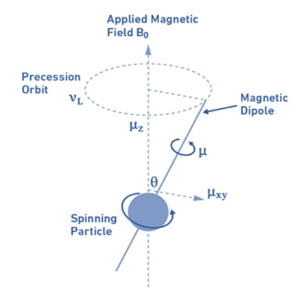
\includegraphics[width=0.5\textwidth]{figures/larmor_precession.jpeg}
    \caption{Larmor precession of a nuclear spin in a magnetic field. © 2025 Science Info, from \cite{science_info}.}
    \label{fig:larmor_precession}
\end{figure}

\section{Spatial Encoding}
